%% ============================================================
%%  SECCIÓN 5 — Materiales y Equipos
%%  Responsable: [Nombre]
%% ============================================================

\section{Materiales y Equipos}

Para la realización del presente experimento se emplearon los siguientes
materiales e instrumentos de medición:

%% --- Material 1 ---
\subsection{Resorte metálico}

\begin{itemize}
    \item \textbf{Descripción y función:} Resorte helicoidal metálico que actúa como
    cuerpo elástico principal del experimento. Al suspenderse verticalmente y someterse
    a cargas crecientes, permite medir la deformación longitudinal y verificar la
    Ley de Hooke dentro del límite elástico.
    \item \textbf{Especificaciones:}
    \begin{itemize}
        \item Longitud natural: $\ell_0 = \qty{16.6 \pm 0.5}{cm}$
        \item Grosor del alambre: $d = \qty{5.50 \pm 0.05}{mm}$
        \item Área de la sección transversal: $S_0 = \pi(d/2)^2 \approx \qty{23.76}{mm^2}$
        \item Masa: $m_{\text{resorte}} = \qty{46.3 \pm 0.5}{g}$
    \end{itemize}
    \item \textbf{Precauciones:} No superar el límite elástico del resorte. Verificar
    que recupere su longitud natural al retirar cada carga antes de continuar.
\end{itemize}

\begin{figure}[H]
    \centering
    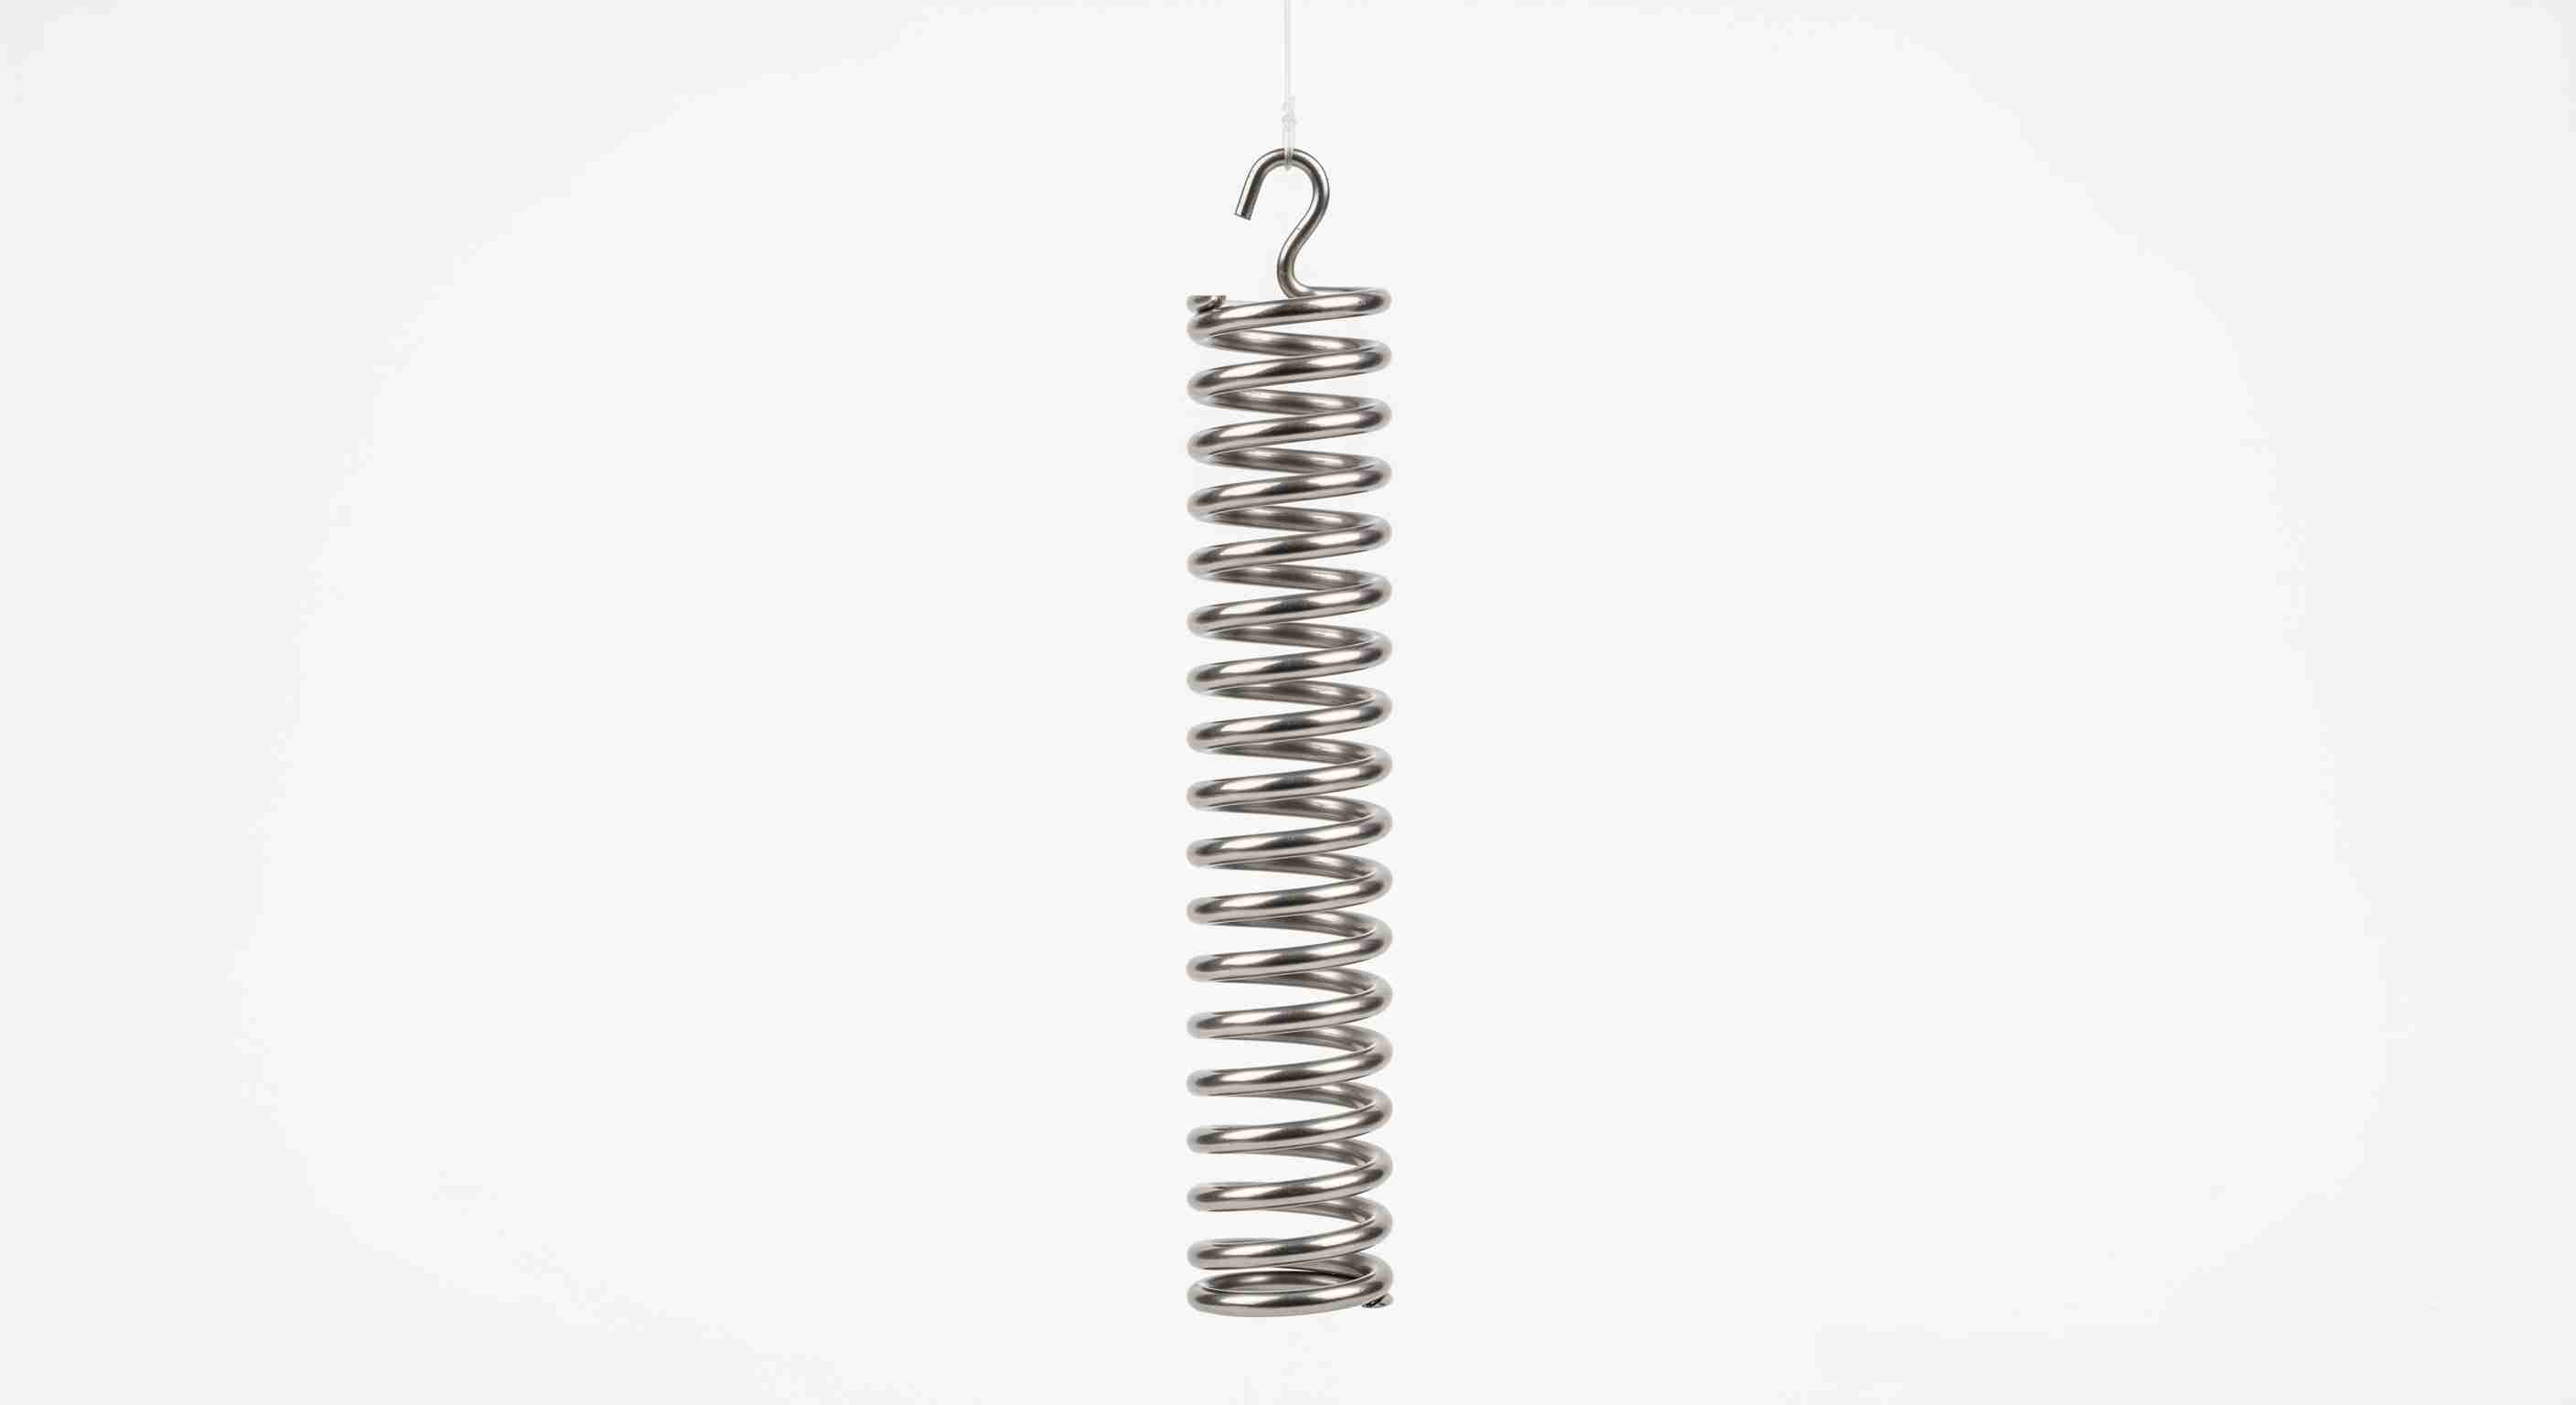
\includegraphics[width=0.40\linewidth]{Figures/resorte.jpg}
    \caption{Resorte metálico empleado como cuerpo elástico en el experimento.}
    \label{fig:resorte}
\end{figure}

%% --- Material 2 ---
\subsection{Liga (tira de jebe)}

\begin{itemize}
    \item \textbf{Descripción y función:} Tira de material elastomérico (jebe) utilizada
    como segundo cuerpo de estudio. A diferencia del resorte, presenta histéresis
    elástica, por lo que las curvas de carga y descarga no coinciden.
    \item \textbf{Especificaciones:}
    \begin{itemize}
        \item Longitud natural: $\ell_0 = \qty{34.2 \pm 0.5}{cm}$
        \item Diámetro de la sección transversal: $d = \qty{14.80 \pm 0.05}{mm}$
        \item Área de la sección transversal: $S_0 = \pi(d/2)^2 \approx \qty{172.03}{mm^2}$
        \item Masa: $m_{\text{liga}} = \qty{40.2 \pm 0.5}{g}$
    \end{itemize}
    \item \textbf{Precauciones:} No aplicar cargas excesivas que deformen
    permanentemente la liga. Las cargas aplicadas deben ser mayores que el peso propio
    del material para garantizar una deformación medible.
\end{itemize}

\begin{figure}[H]
    \centering
    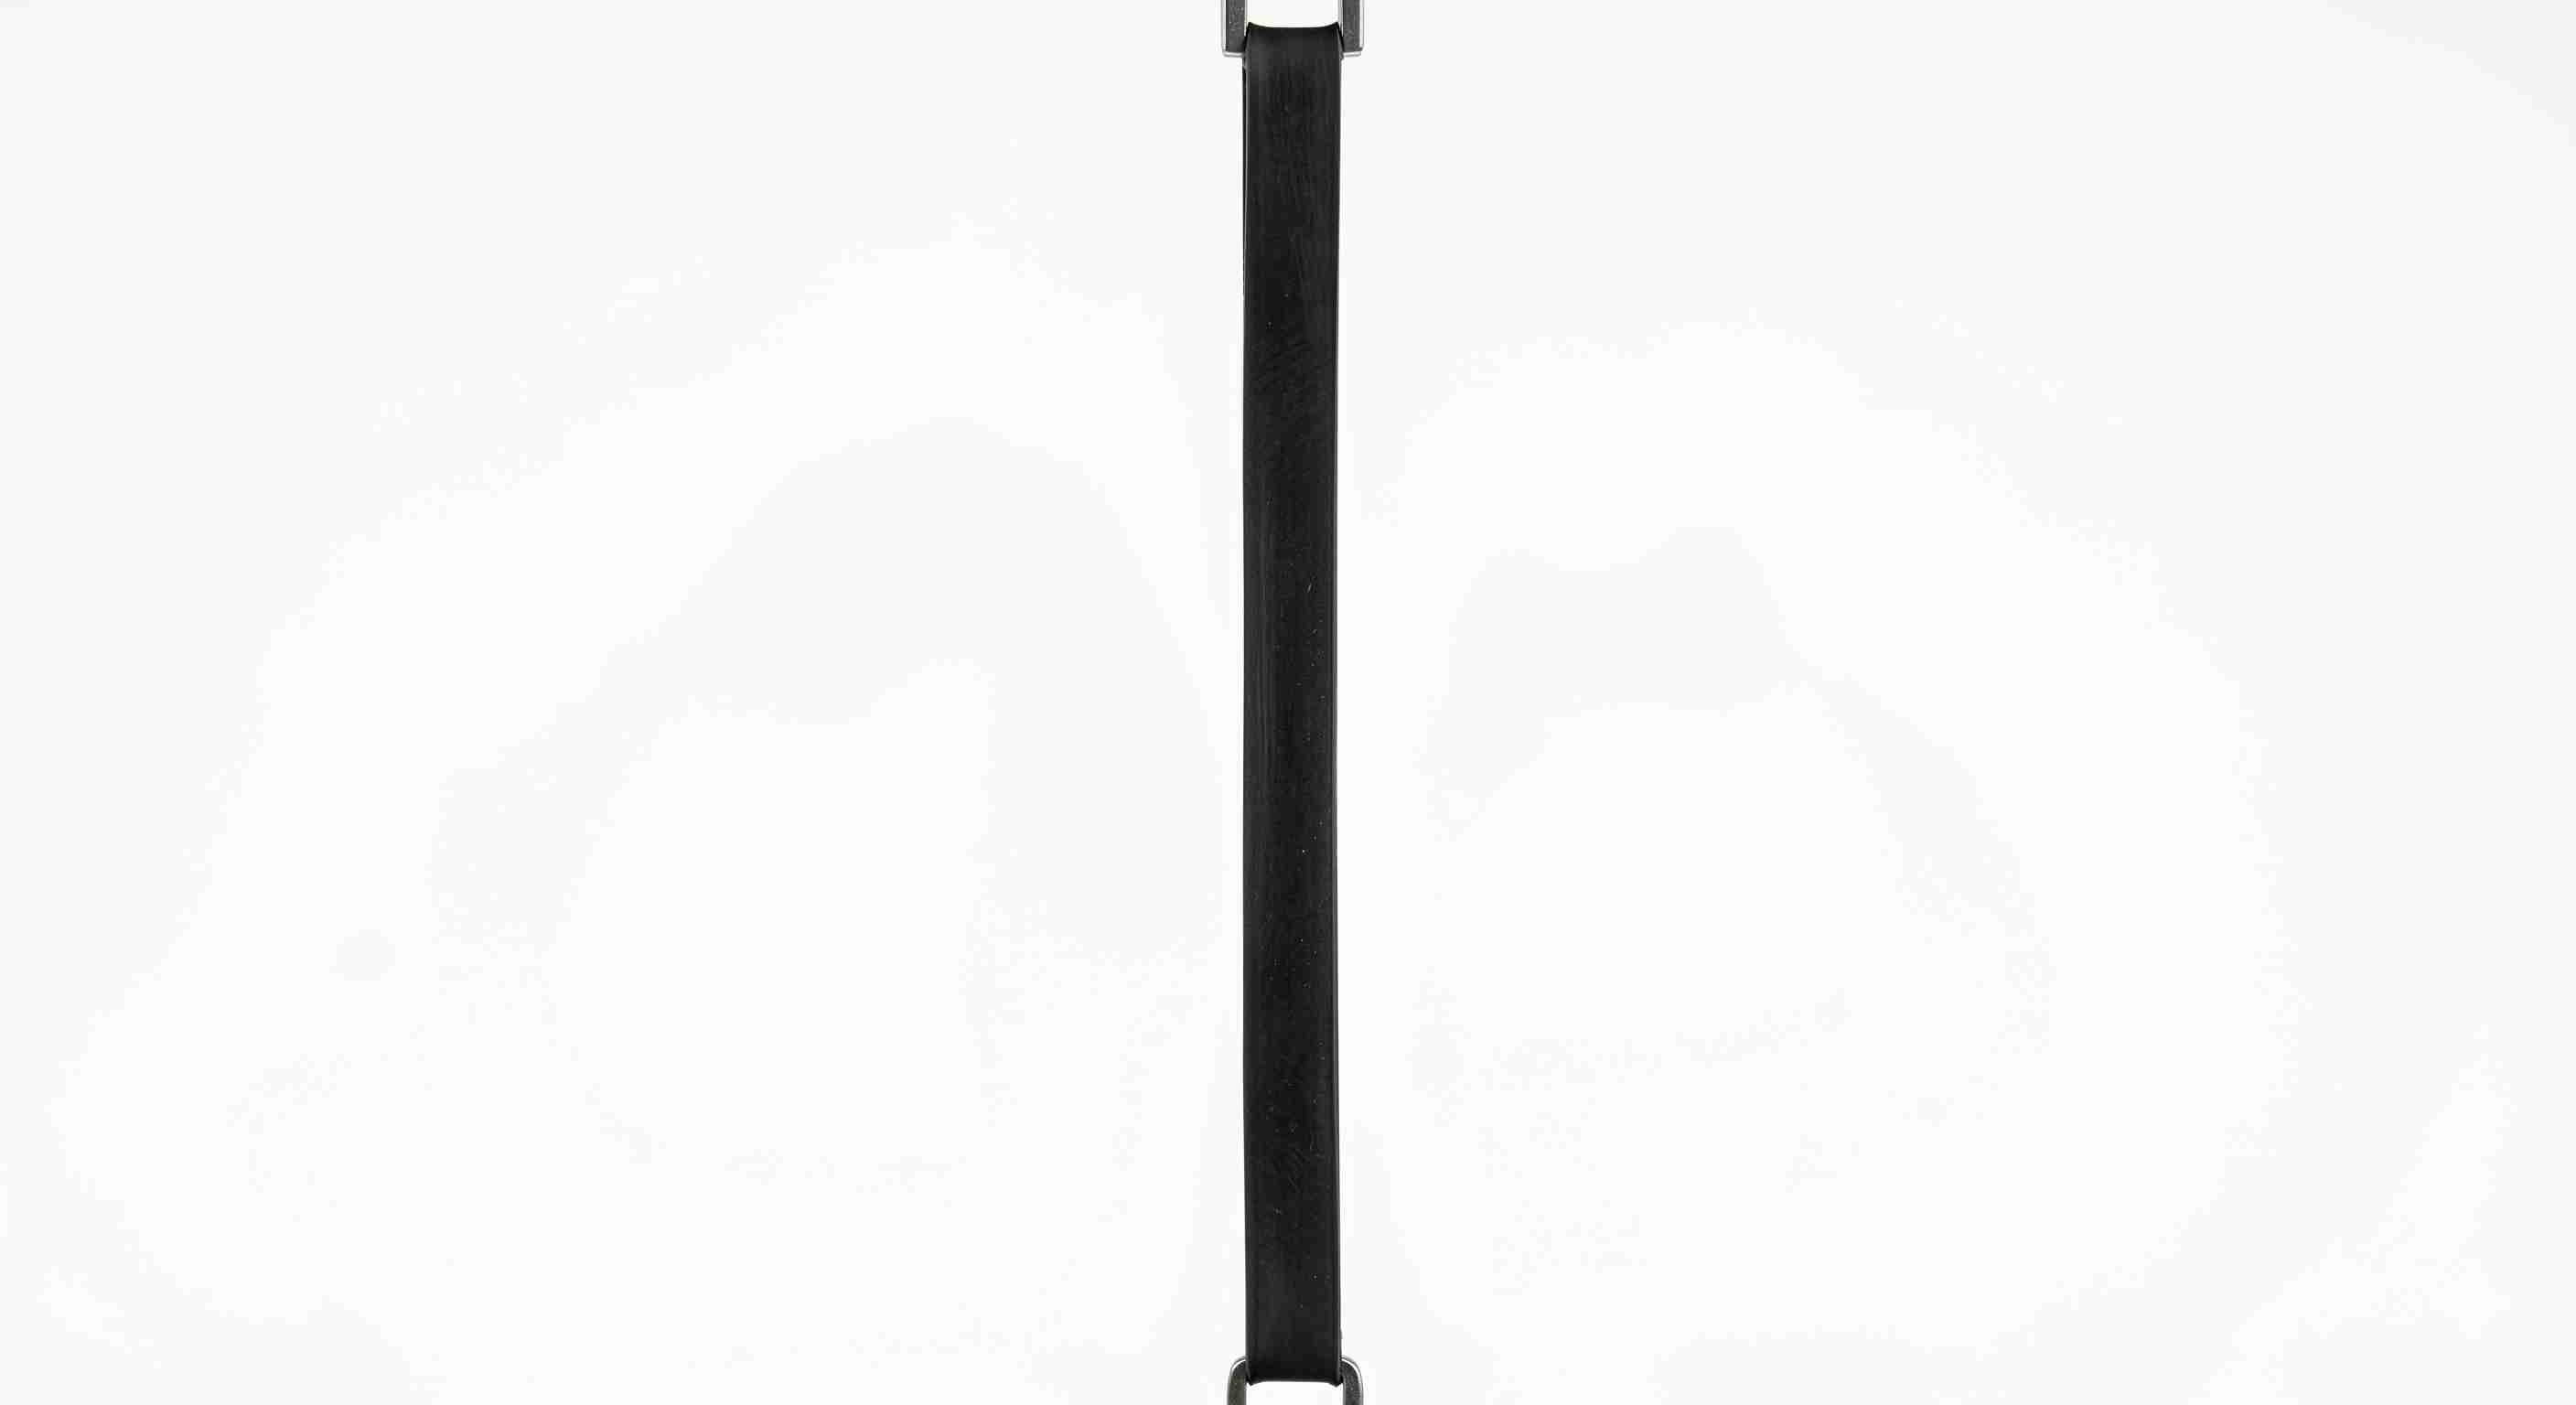
\includegraphics[width=0.40\linewidth]{Figures/liga.jpg}
    \caption{Tira de jebe (liga) utilizada como material no perfectamente elástico.}
    \label{fig:liga}
\end{figure}

%% --- Instrumento 1 ---
\subsection{Regla métrica}

\begin{itemize}
    \item \textbf{Descripción y función:} Instrumento de medición lineal utilizado para
    determinar la longitud natural $\ell_0$ y la longitud deformada $\ell$ del resorte
    y la liga bajo cada carga aplicada.
    \item \textbf{Especificaciones:}
    \begin{itemize}
        \item Resolución: \qty{1}{mm}
        \item Incertidumbre: \qty{\pm 0.5}{mm}
    \end{itemize}
    \item \textbf{Precauciones:} Realizar las mediciones con el material en reposo y
    alineado verticalmente. Minimizar errores de paralaje.
\end{itemize}

\begin{figure}[H]
    \centering
    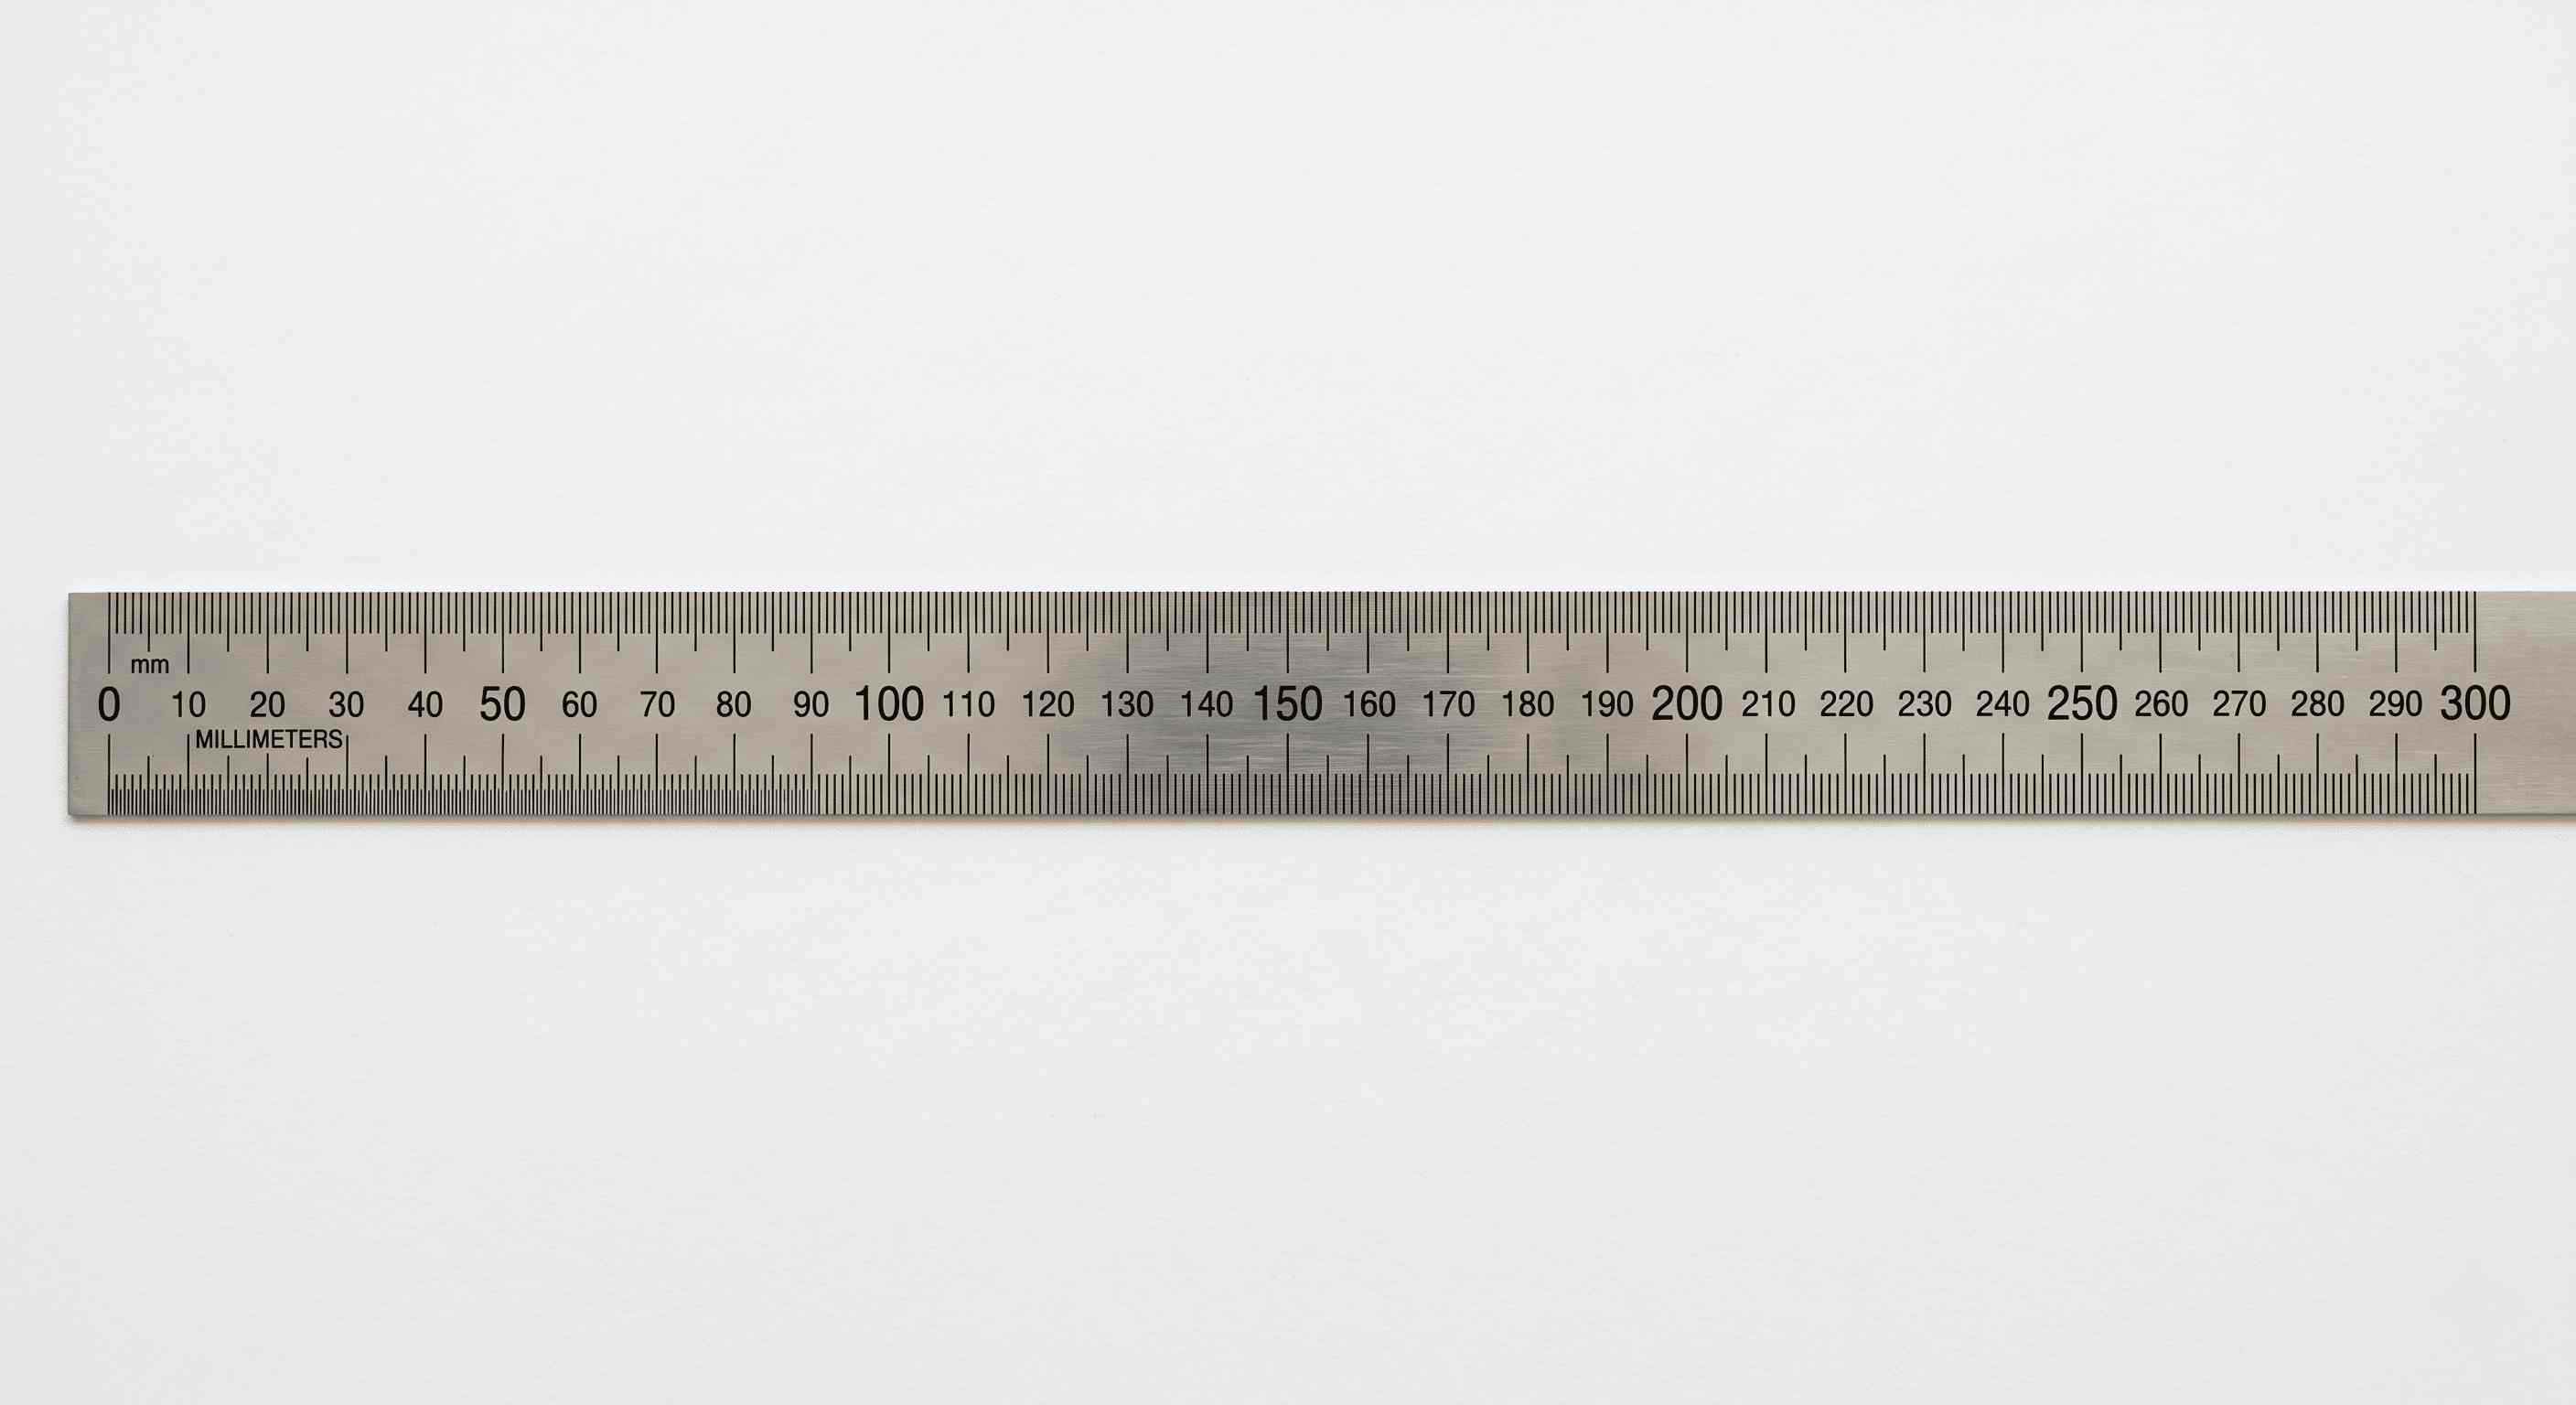
\includegraphics[width=0.55\linewidth]{Figures/regla.jpg}
    \caption{Regla métrica empleada para la medición de longitudes.}
    \label{fig:regla}
\end{figure}

%% --- Instrumento 2 ---
\subsection{Vernier (calibrador)}

\begin{itemize}
    \item \textbf{Descripción y función:} Instrumento utilizado para medir el diámetro
    de la sección transversal del resorte (\qty{5.50}{mm}) y de la liga (\qty{14.80}{mm}),
    tanto en estado natural como bajo deformación.
    \item \textbf{Especificaciones:}
    \begin{itemize}
        \item Resolución: \qty{0.05}{mm}
        \item Incertidumbre: \qty{\pm 0.05}{mm}
    \end{itemize}
    \item \textbf{Precauciones:} Verificar el cero del vernier antes de cada medición.
    Medir siempre en la parte media de la longitud del material.
\end{itemize}

\begin{figure}[H]
    \centering
    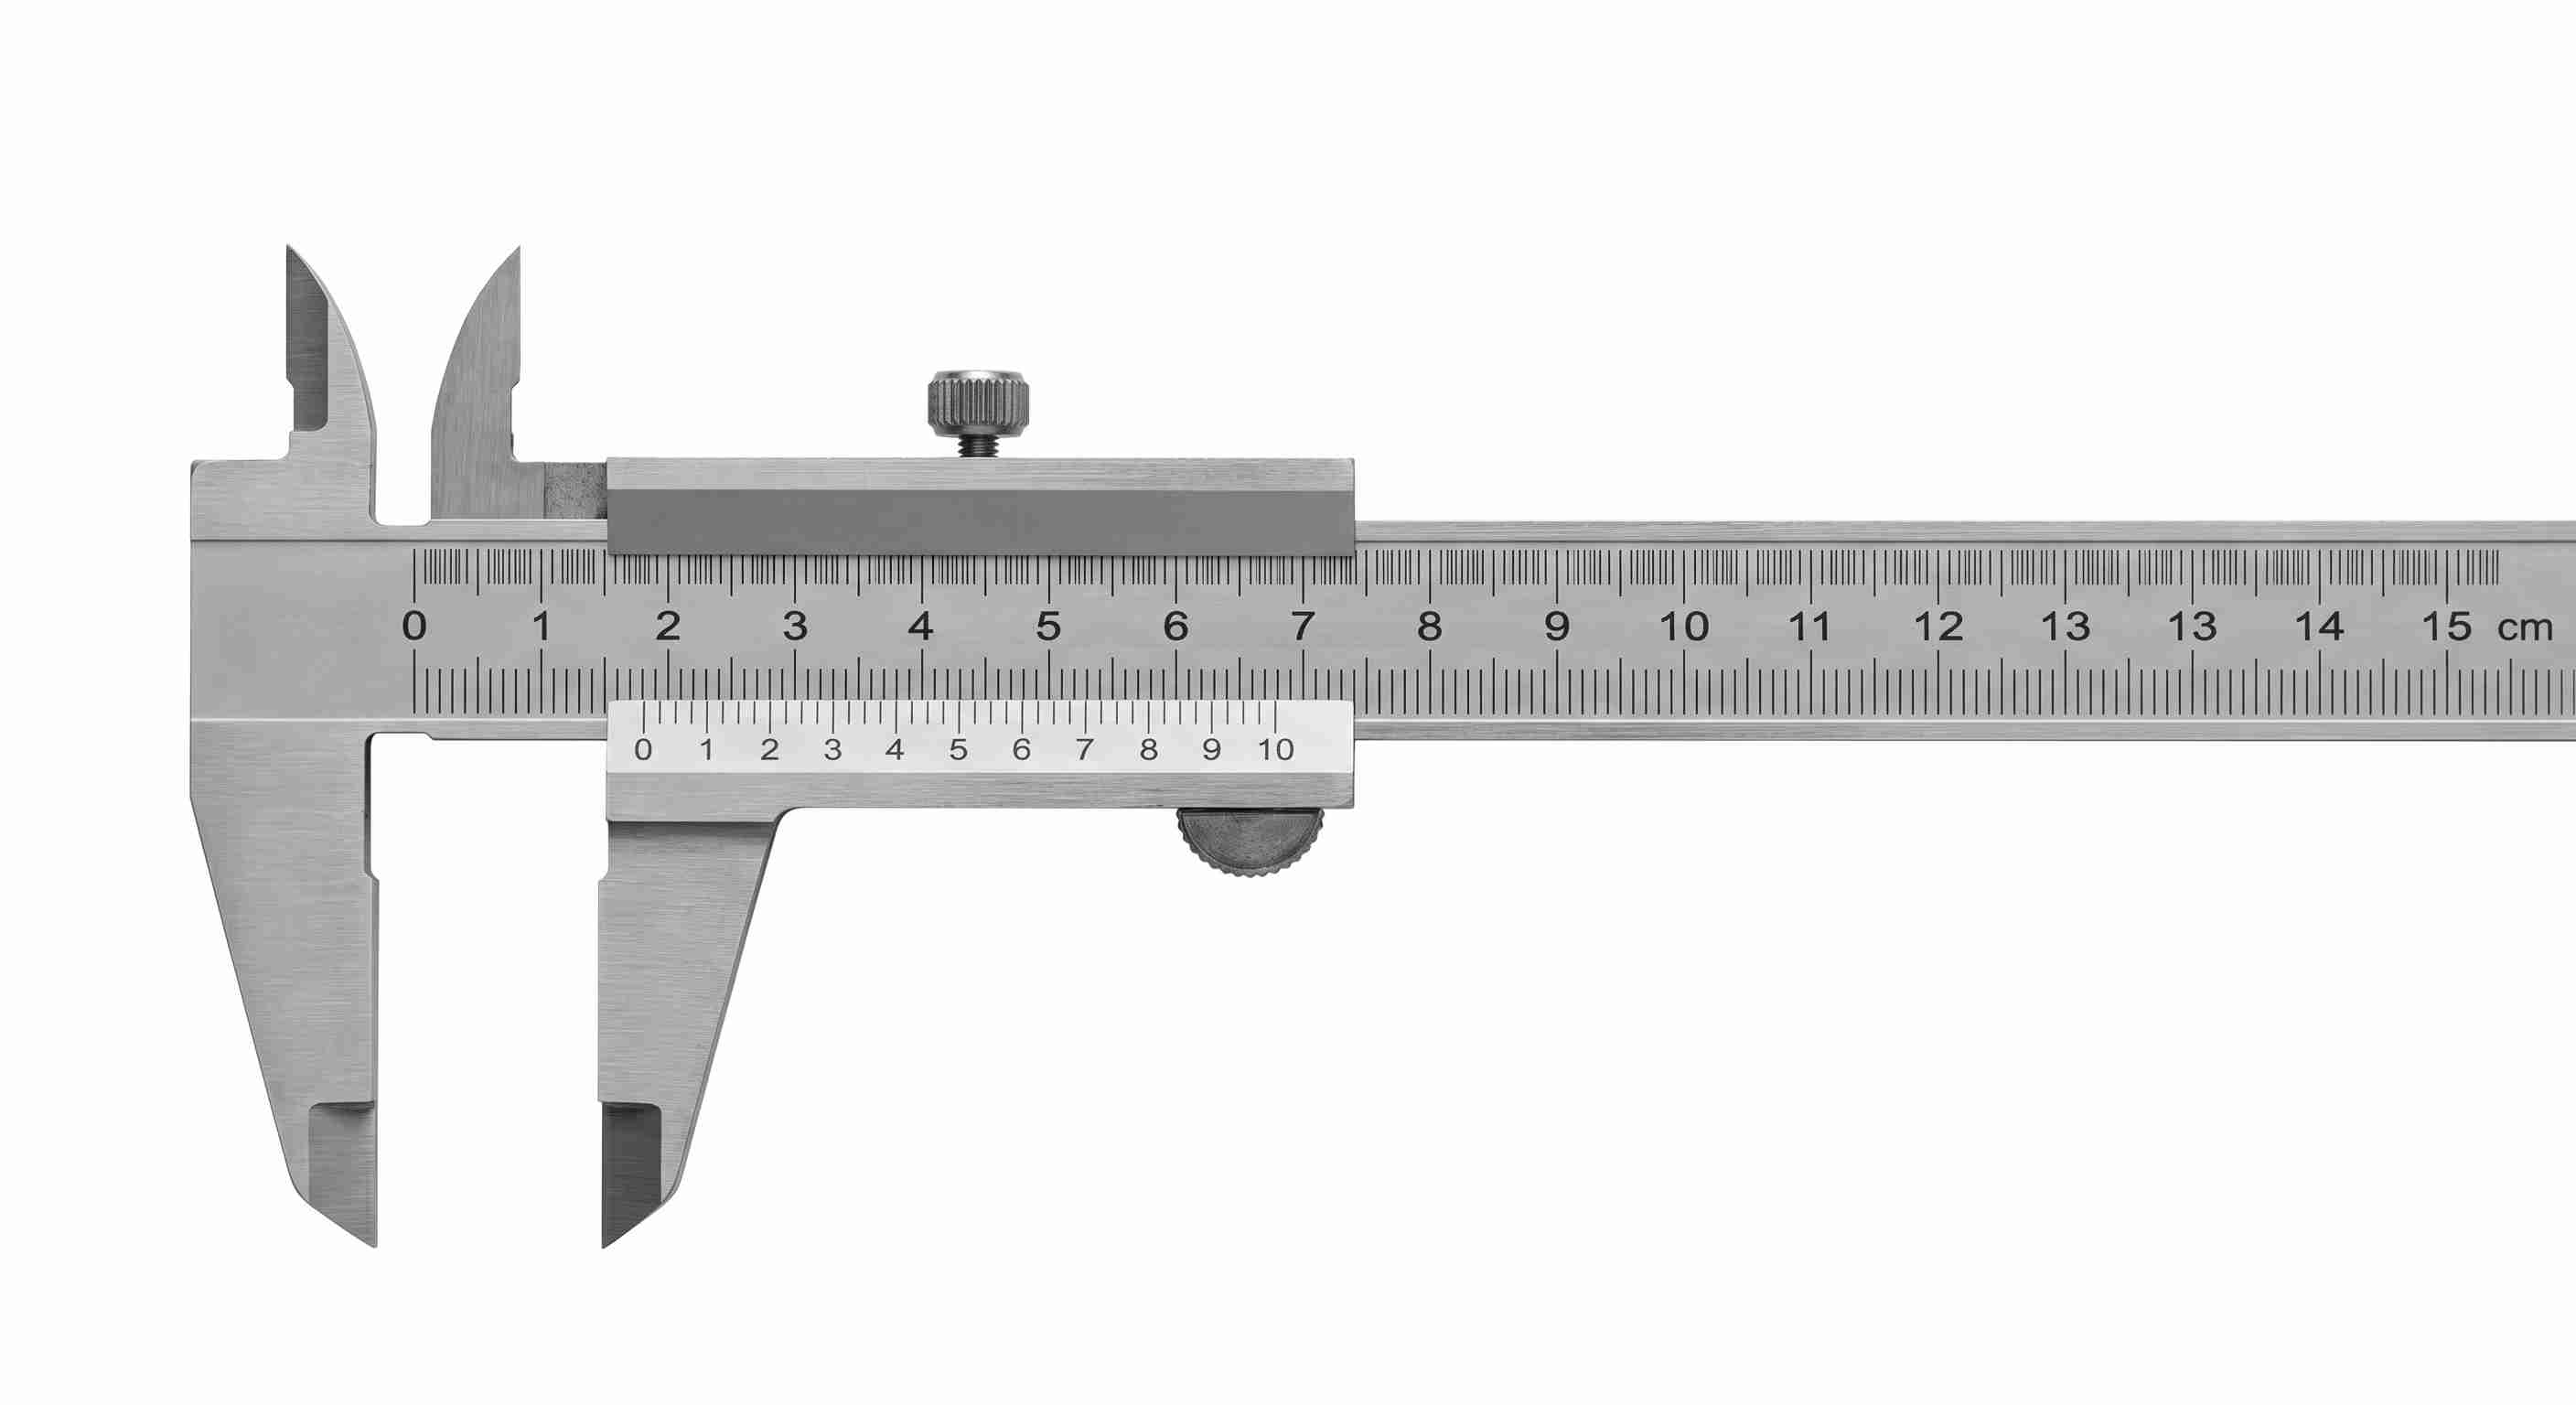
\includegraphics[width=0.50\linewidth]{Figures/vernier.jpg}
    \caption{Vernier (calibrador) empleado para la medición de diámetros.}
    \label{fig:vernier}
\end{figure}

%% --- Instrumento 3 ---
\subsection{Balanza}

\begin{itemize}
    \item \textbf{Descripción y función:} Instrumento utilizado para determinar la masa
    del resorte, la liga y las cargas aplicadas.
    \item \textbf{Especificaciones:}
    \begin{itemize}
        \item Incertidumbre: \qty{\pm 0.5}{g}
    \end{itemize}
    \item \textbf{Precauciones:} Nivelar la balanza antes de cada uso. Instrumento
    compartido por toda la clase; coordinar el turno de medición.
\end{itemize}

\begin{figure}[H]
    \centering
    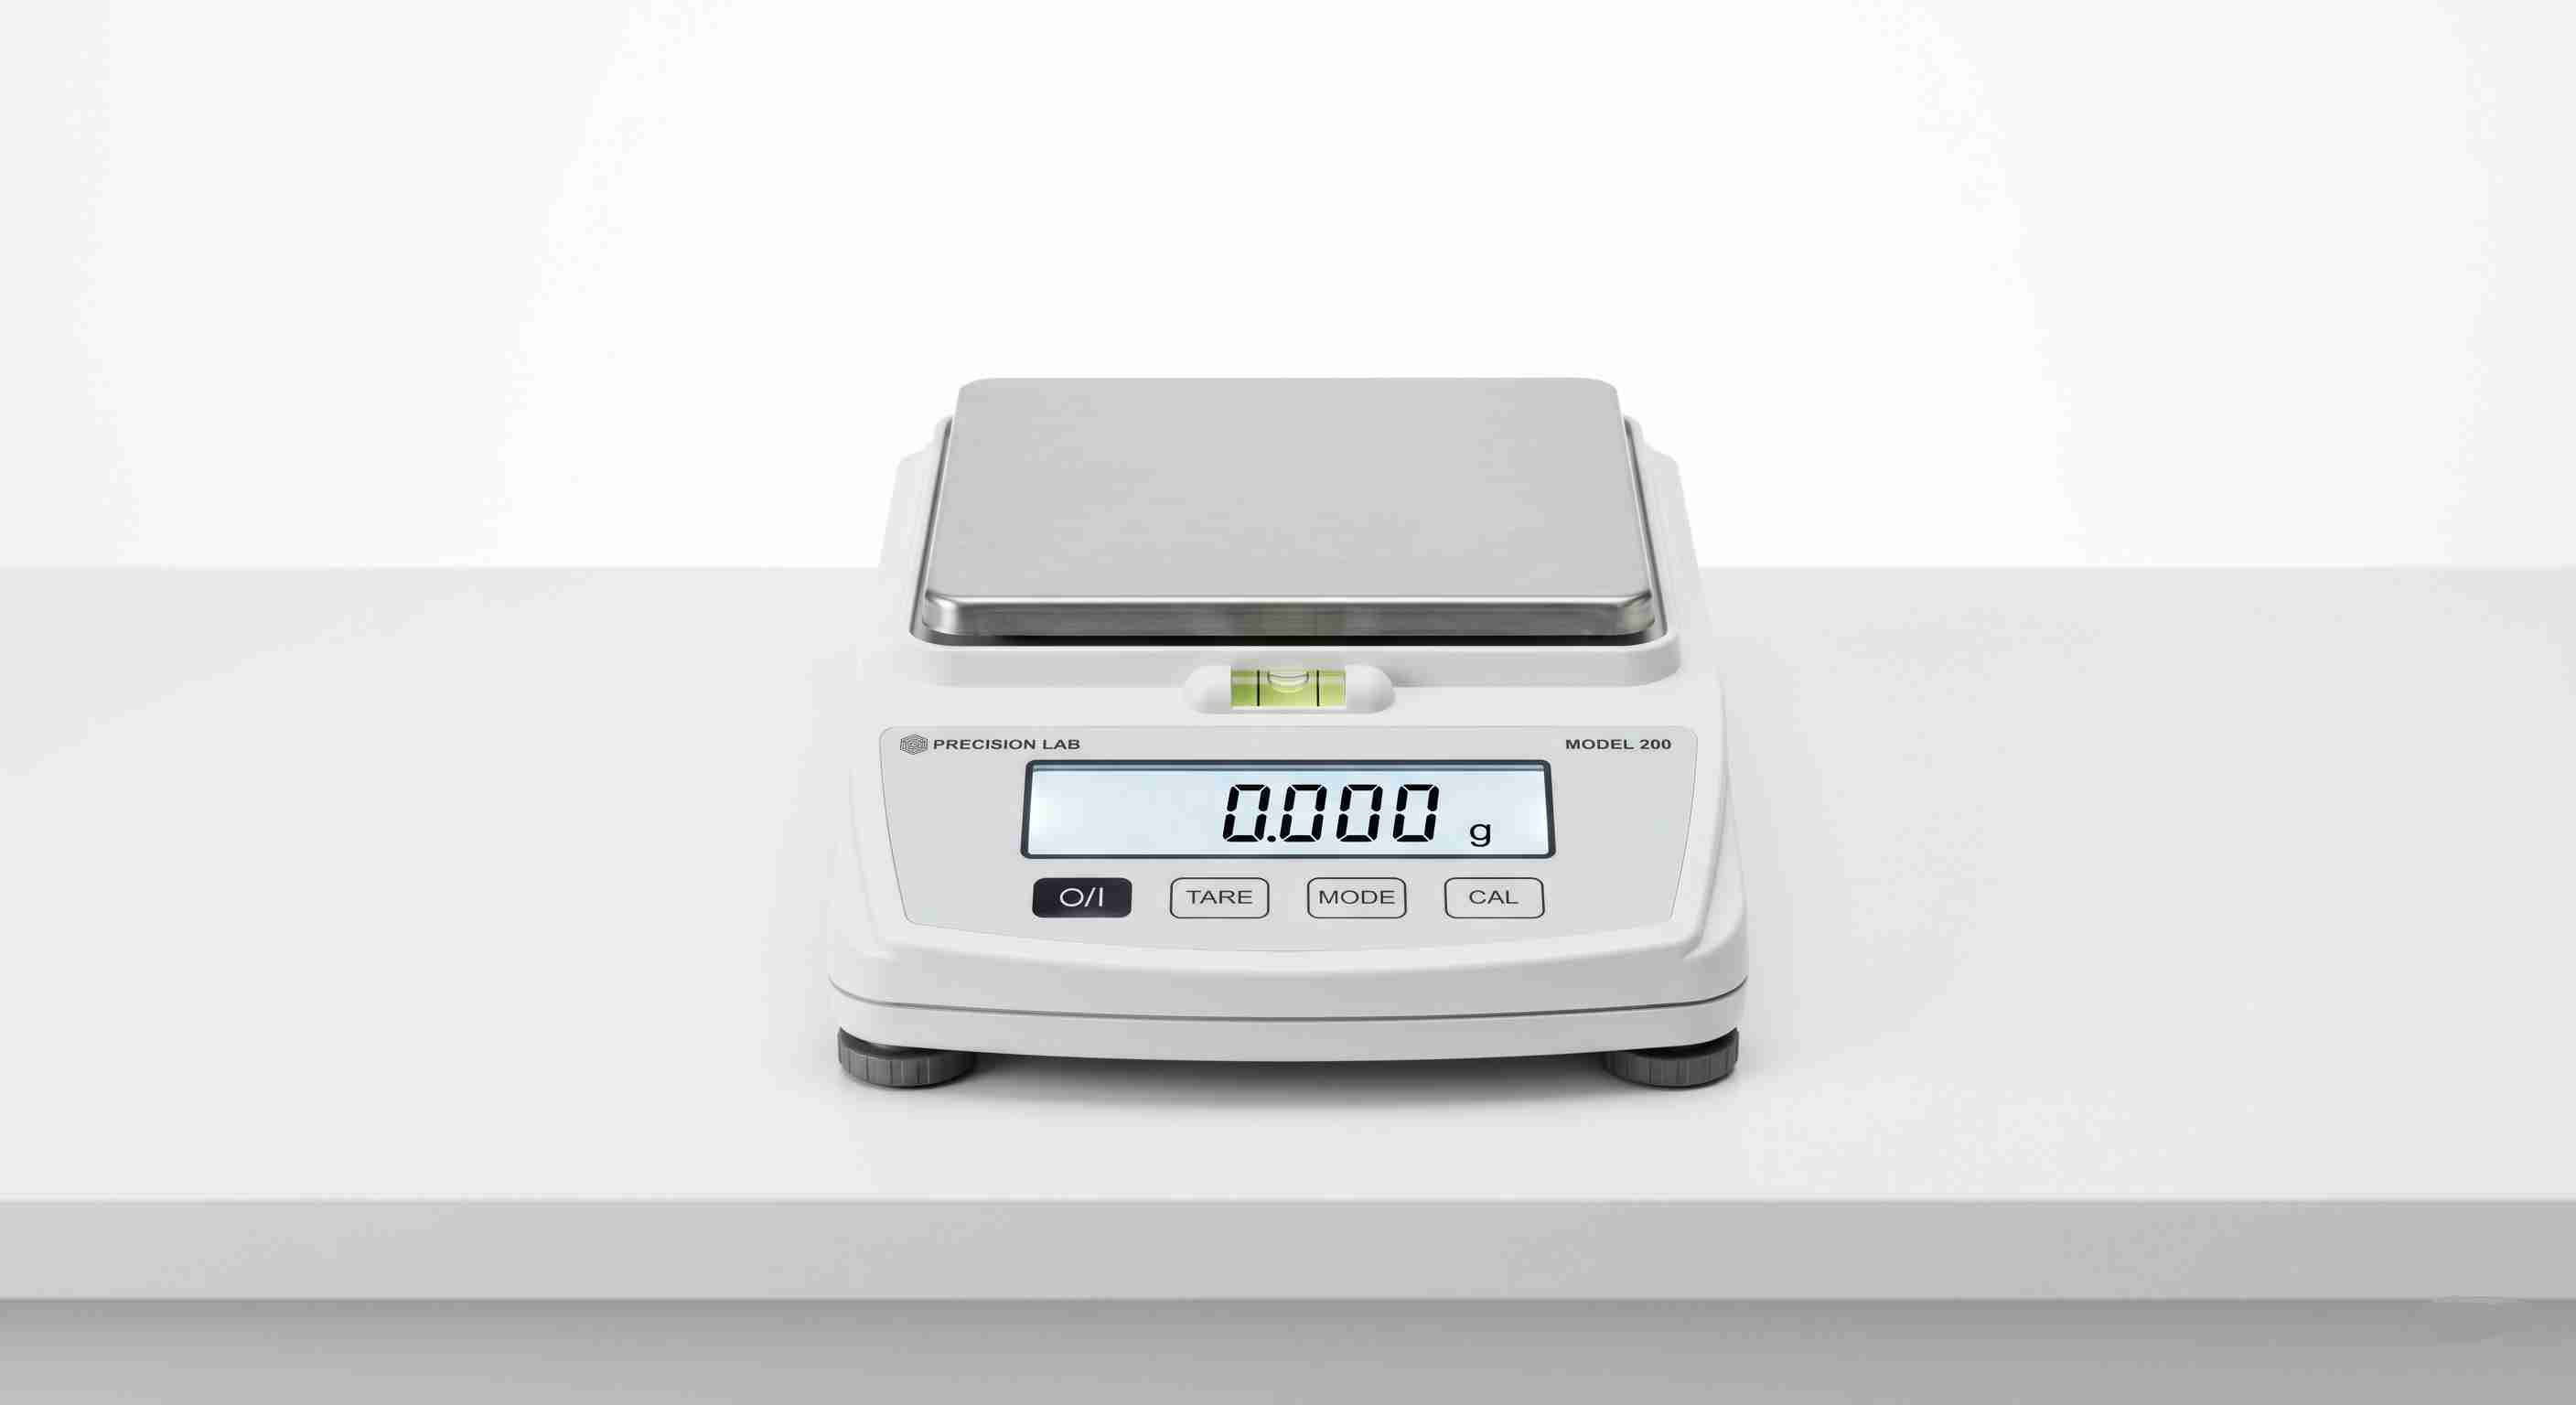
\includegraphics[width=0.45\linewidth]{Figures/balanza.jpg}
    \caption{Balanza empleada para la medición de masas.}
    \label{fig:balanza}
\end{figure}

%% --- Instrumento 4 ---
\subsection{Soporte universal}

\begin{itemize}
    \item \textbf{Descripción y función:} Estructura metálica rígida que sirve de
    base para suspender verticalmente el resorte y la liga, permitiendo su libre
    deformación bajo la acción de las cargas.
    \item \textbf{Precauciones:} Asegurar la estabilidad del soporte antes de colgar
    cualquier masa. Verificar que el material quede perfectamente vertical.
\end{itemize}

\begin{figure}[H]
    \centering
    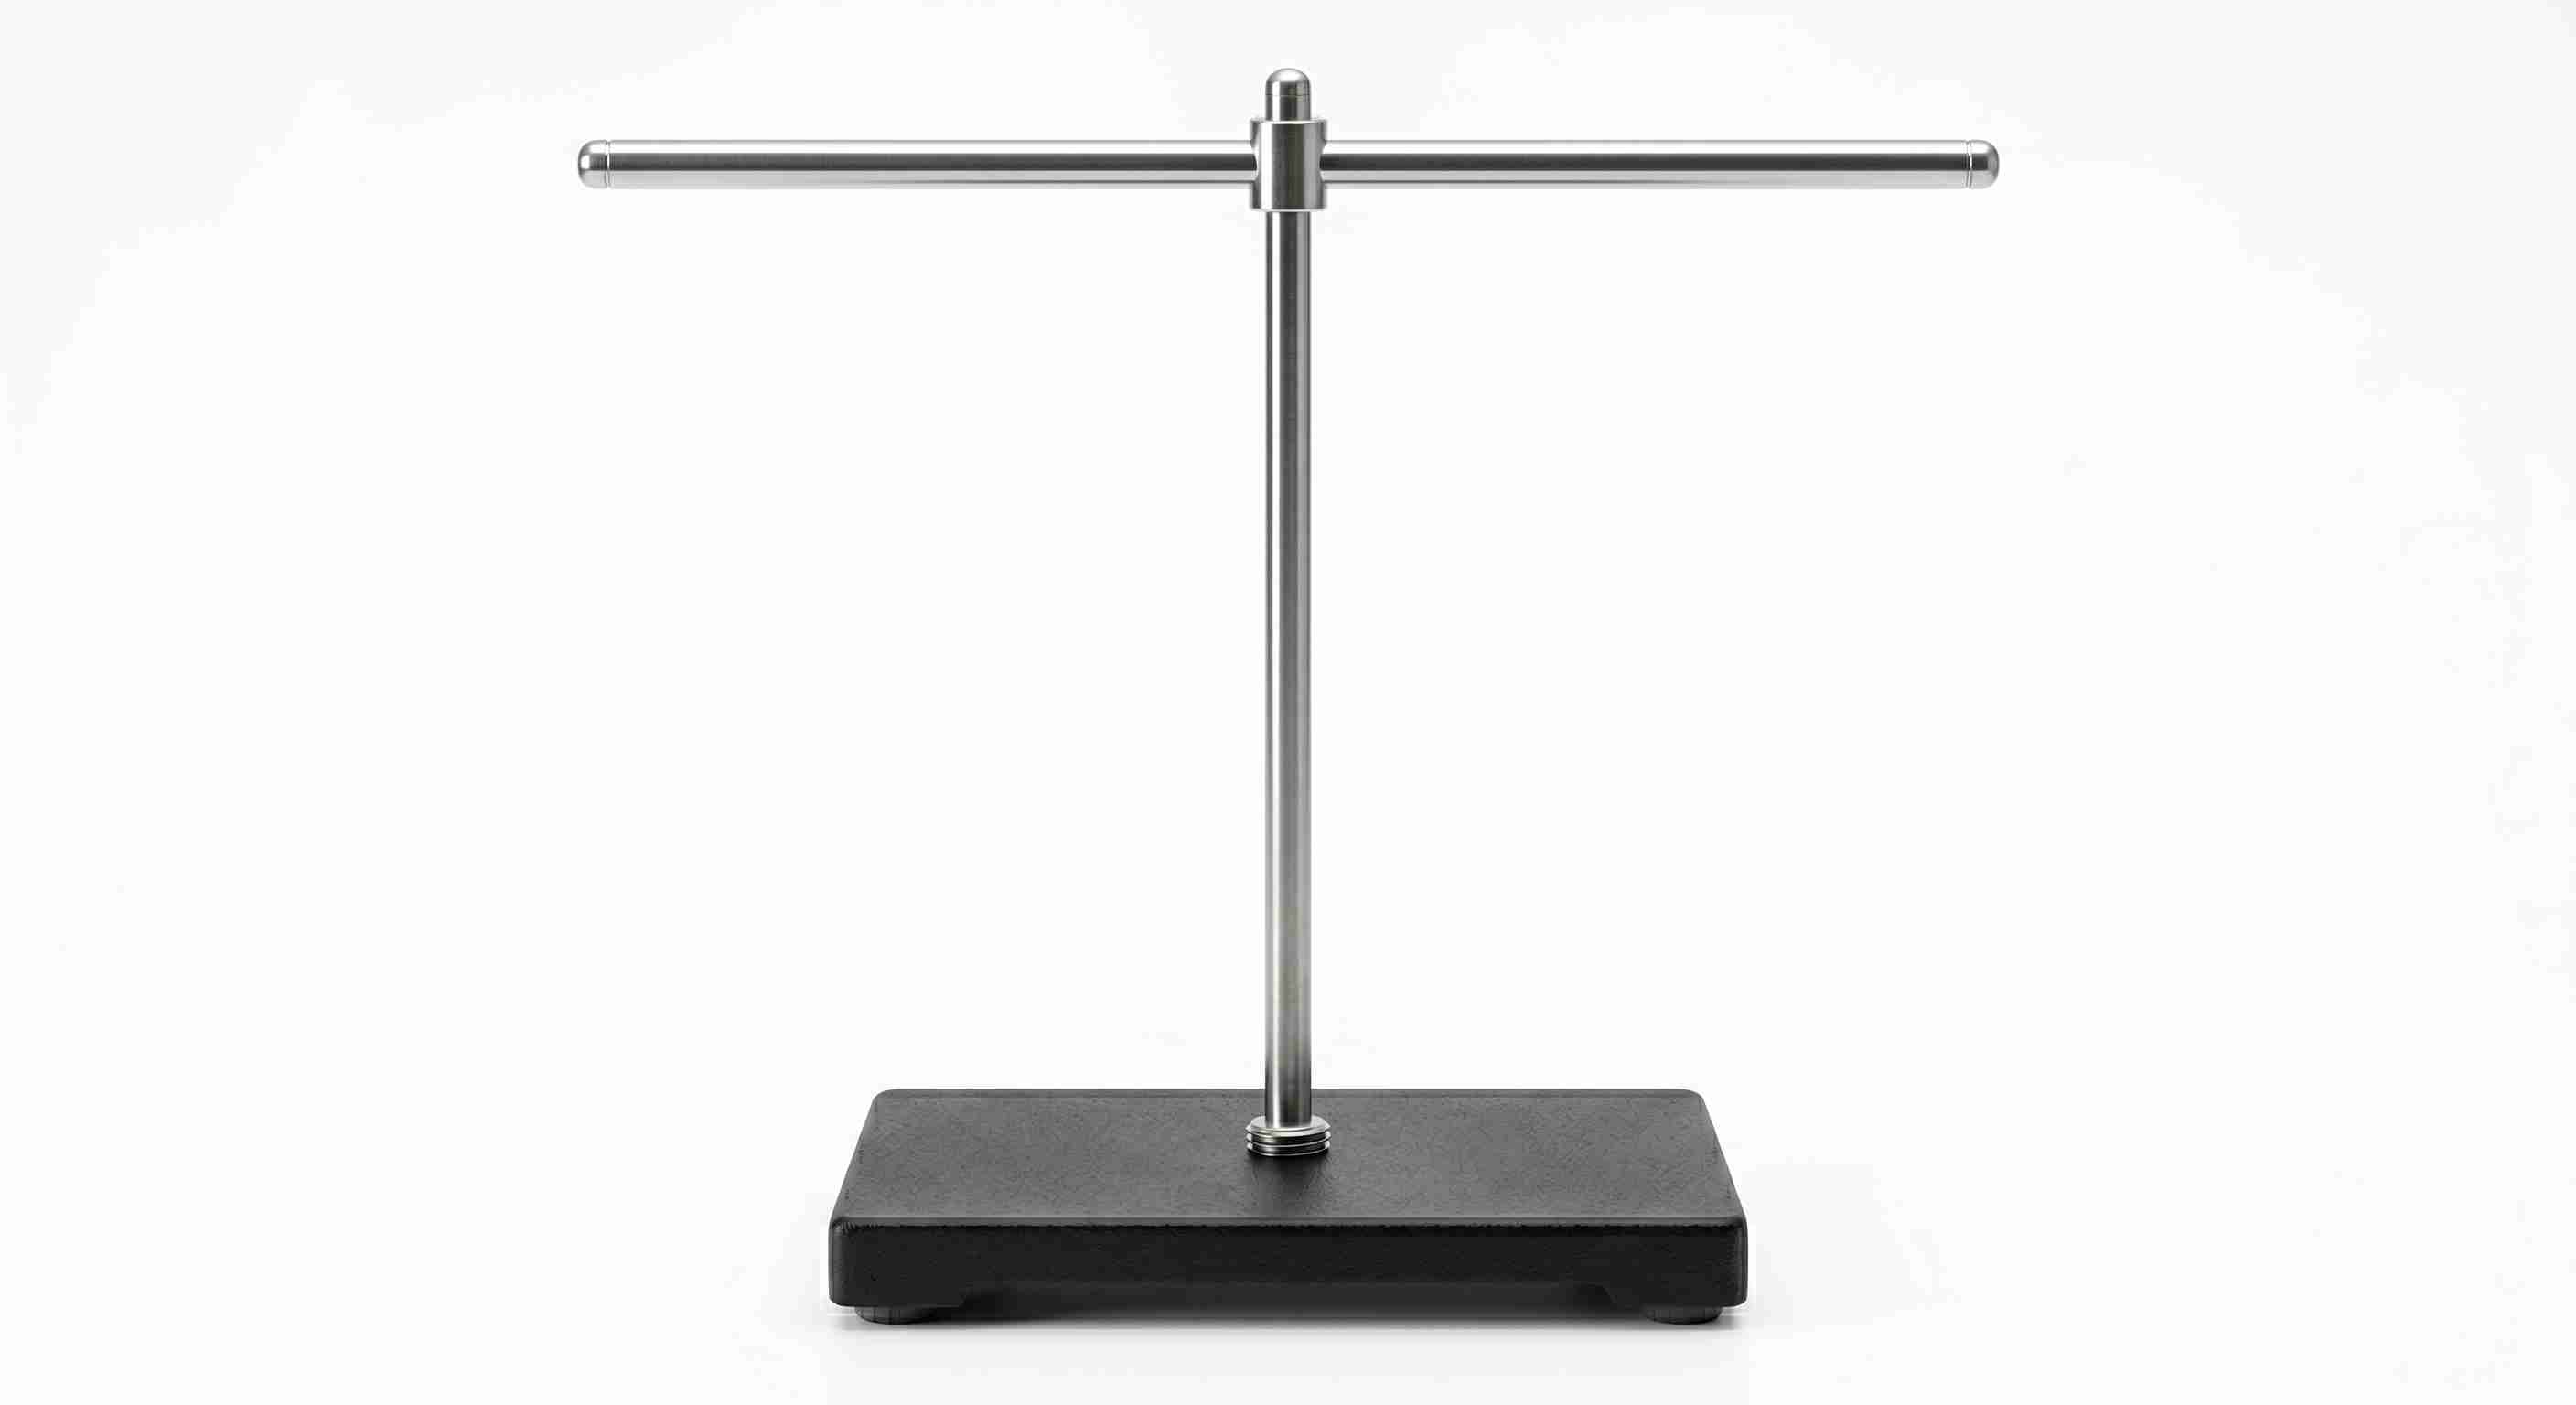
\includegraphics[width=0.40\linewidth]{Figures/soporte.jpg}
    \caption{Soporte universal utilizado para suspender los materiales de estudio.}
    \label{fig:soporte}
\end{figure}

%% --- Material 3 ---
\subsection{Masas de calibración}

\begin{itemize}
    \item \textbf{Descripción y función:} Conjunto de cuatro masas de valores nominales
    conocidos, utilizadas para aplicar cargas crecientes de forma acumulativa sobre el
    resorte y la liga.
    \item \textbf{Especificaciones:}
    \begin{itemize}
        \item $m_1$: nominal \qty{250}{g}, \quad masa real $= \qty{254.5 \pm 0.5}{g}$,
              \quad $P_1 = \qty{2.497}{N}$
        \item $m_2$: nominal \qty{250}{g}, \quad masa real $= \qty{253.7 \pm 0.5}{g}$,
              \quad $P_2 = \qty{2.489}{N}$
        \item $m_3$: nominal \qty{500}{g}, \quad masa real $= \qty{499.8 \pm 0.5}{g}$,
              \quad $P_3 = \qty{4.903}{N}$
        \item $m_4$: nominal \qty{1000}{g}, \quad masa real $= \qty{1005.0 \pm 0.5}{g}$,
              \quad $P_4 = \qty{9.859}{N}$
    \end{itemize}
    \item \textbf{Precauciones:} Colocar y retirar las masas suavemente para evitar
    oscilaciones. Las cargas se aplican de forma acumulativa sin retirar las anteriores,
    y se retiran en orden inverso durante la descarga.
\end{itemize}

\begin{figure}[H]
    \centering
    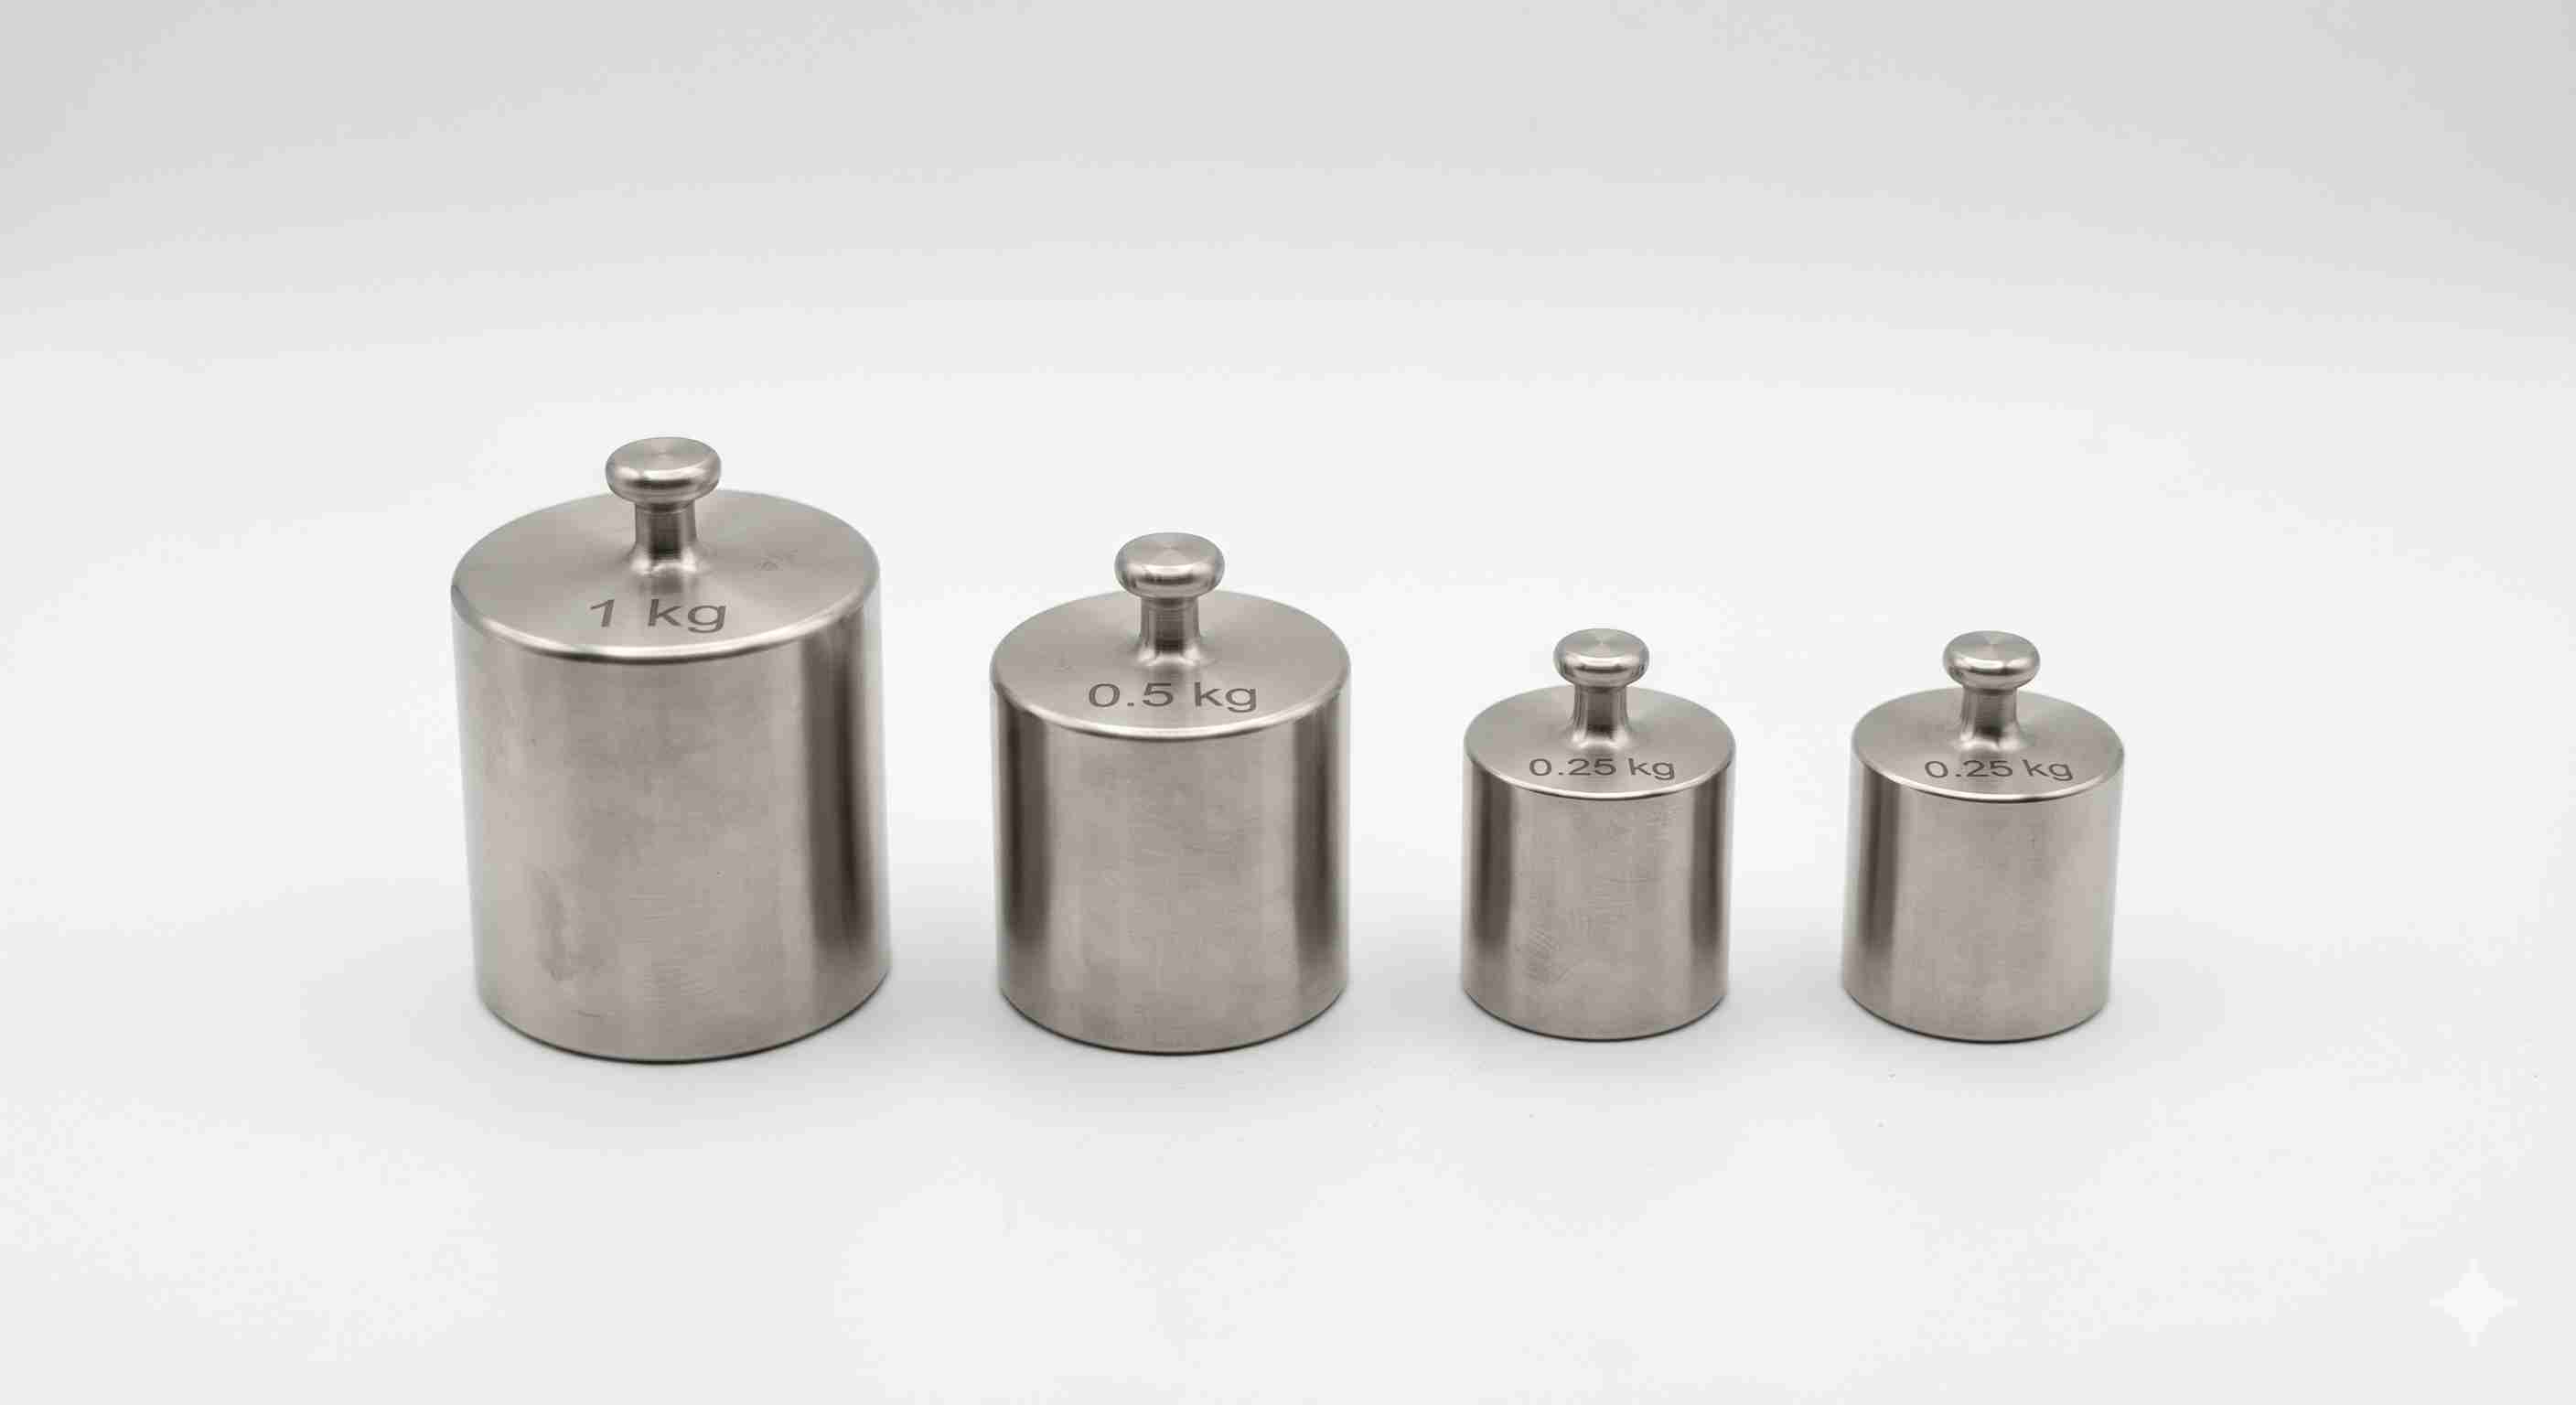
\includegraphics[width=0.40\linewidth]{Figures/masas.jpg}
    \caption{Masas de calibración empleadas para aplicar las cargas sobre los materiales.}
    \label{fig:masas}
\end{figure}